\documentclass{beamer}
\usepackage{graphicx}
\usepackage{caption}
\usepackage{subcaption}
\captionsetup{compatibility=false}
%\usepackage[italian]{babel}  

%% Se per qualsiasi motivo non riuscissi a compilare col tema Unipd,
%% basta commentare la riga qui sotto e si passa automaticamente al
%% tema beamer di default.
\usetheme{Unipd}

\title{Co-Simulazione di un sistema controllato da microprocessori}
%\subtitle{da inserire}
\author{Diego Casella, Fabio Marcuzzi, Paolo Martin}
\date{\today}

\begin{document}

\maketitle

\begin{frame}{Contenuti} %Outline
\tableofcontents
\end{frame}

%% Introduzione
\section{Introduzione}
\begin{frame}{Introduzione}
Com'\'e accaduto ormai da parecchio tempo in vari settori dell'ingegneria (civile, aerospaziale, meccanica),
anche per l'ingegneria dei sistemi di controllo la prototipazione virtuale \'e diventata una metodologia
possibile e desiderabile, quando non addirittura necessaria. 

\bigskip

Mediante la simulazione numerica del sistema controllato \'e possibile studiare il funzionamento del sistema
con una risoluzione temporale impensabile nella sperimentazione fisica, ed analizzare il sistema dal punto di vista:
\begin{itemize}
\item dell'interazione tra firmware e sistema fisico;
\item dell'analisi numerica degli algoritmi implementati nel firmware.
\end{itemize}


\end{frame}

%% Microcontrollori/DSP
\section{Microcontrollori/DSP}
\begin{frame}{Microcontrollori/DSP}
\begin{figure}
\centering
\begin{subfigure}{.5\textwidth}
  \centering
  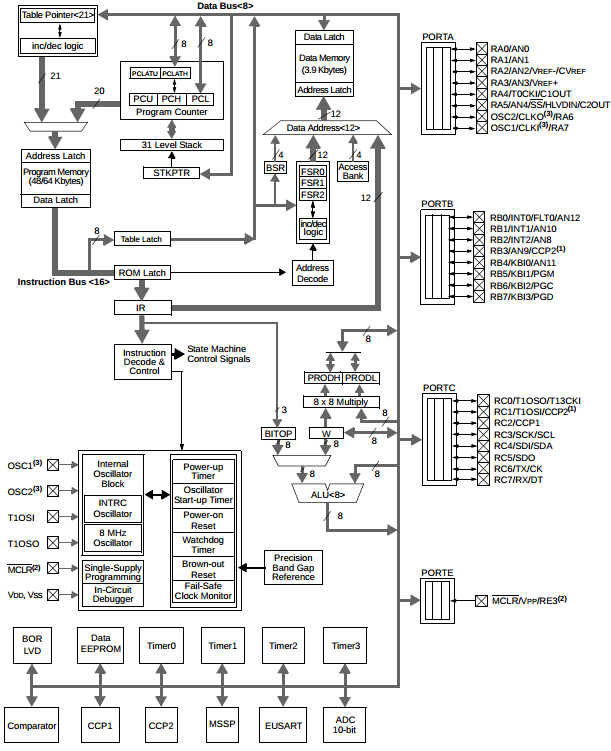
\includegraphics[scale=0.35]{images/pic18f4620.png}
  \caption{Schema interno}
\end{subfigure}%
\begin{subfigure}{.5\textwidth}
  \centering
  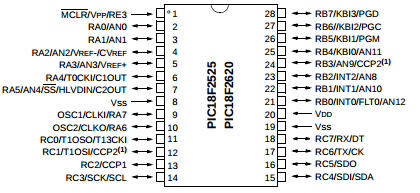
\includegraphics[scale=0.4]{images/pic18f4620_pinout.png}
  \caption{Pinout fisico}
\end{subfigure}
%\caption{Visione d'insieme del device PIC18F4620}
\end{figure}
\end{frame}

\begin{frame}{Microcontrollori/DSP}
\begin{itemize}
{\small
\item Esistono moltissime varianti di questi dispositivi: diciamo almeno 10 produttori con circa 1000 dispositivi ciascuno.
\item Relativamente pochi dispositivi (alcune decine) condividono la stessa CPU (8-16-32 bit, vari set di istruzioni, es. DSP).
\item Pochissimi dispositivi (al massimo poche decine) condividono le stesse periferiche, che per numerosit\'a variano comunque da dispositivo a dispositivo.
\item Il progetto del sistema di controllo \'e legato alle specifiche periferiche (tipologia e numerosit\'a) presenti nel dispositivo.
\item Il firmware interagisce direttamente con le periferiche (i sistemi operativi generalisti non sono quasi mai usati nei microcontrollori) e 
pu\'o dunque girare quasi esclusivamente sul singolo dispositivo scelto: la portabilit\'a del firmware \'e molto bassa.
}
\end{itemize}


$\rightarrow$ \textbf{la co-simulazione richiede il simulatore dello specifico dispositivo utilizzato}.
\end{frame}

\begin{frame}{Microcontrollori/DSP}
Ogni microcontrollore \'e una macchina complessa: il suo reale funzionamento dipende dai valori programmati in una moltitudine
di registri che governano le periferiche.

\bigskip

$\rightarrow$ \textbf{Il simulatore \'e un software complesso ed impegnativo da debuggare}.
\end{frame}

\begin{frame}{Microcontrollori/DSP}
Il funzionamento fisico interno del microcontrollore non \'e oggetto della co-simulazione, viene dato per buono; viene simulato il funzionamento logico.

\bigskip

Il modello del sistema di controllo e del sistema multifisico controllato hanno invece significato fisico e quindi viene simulato il loro
funzionamento fisico. Il confine tra modello logico e fisico \'e il pinout del microcontrollore, dove i livelli logici diventano
livelli di tensione elettrica.
\end{frame}

\begin{frame}{Microcontrollori/DSP}
La velocit\'a di funzionamento \'e una questione fondamentale: sono macchine RISC con clock 5-40 MHz e quindi la complessit\'a computazionale
del simulatore \'e elevata.

\bigskip

Non \'e possibile parallelizzare una singola esecuzione del firmware.
\end{frame}

\section{Co-simulazione}
\begin{frame}{Co-simulazione}
Queste criticit\'a fanno s\'i che realizzare un simulatore performante \'e uno sforzo notevole e gestire la diversificazione
lo \'e ancor di pi\'u.

\bigskip

Inoltre, un simulatore ha senso se pu\'o essere usato in modo friendly: deve essere ben integrato con il progetto firmware
e quindi con il suo ambiente di sviluppo, ed avere una buona GUI.

\bigskip

$\rightarrow$ \textbf{Questi ultimi aspetti fanno preferire Java come linguaggio per lo sviluppo di simulatori, mentre questioni di performance
indicherebbero il C come ottimale}.
\end{frame}

\begin{frame}{Co-simulazione}
Java difatti permette una rapida realizzazione dell'idea di simulatore che si ha in mente, permettendo allo sviluppatore di
focalizzarsi sull'architettura dell'implementazione. 

\bigskip

$\rightarrow$ Ci\'o non esclude il fatto che, una volta realizzato il simulatore e delineata la sua struttura funzionale, esso
non possa essere reimplementato in linguaggi pi\'u performanti come C/C++.
\end{frame}

\begin{frame}{Co-simulazione}
Un altro requisito che la co-simulazione impone \'e il controllo fine del simulatore: non \'e sufficiente avviare il simulatore ed
attendere l'ottenimento dell'andamento dei pin a simulazione conclusa, bens\'i:
\begin{itemize}
  \item conoscere i valori assunti dai registri/memorie (debugging, tracing variabili)
\end{itemize}
\end{frame}

\begin{frame}{Co-simulazione}
Un altro requisito che la co-simulazione impone \'e il controllo fine del simulatore: non \'e sufficiente avviare il simulatore ed
attendere l'ottenimento dell'andamento dei pin a simulazione conclusa, bens\'i:
\begin{itemize}
  \item  modificare il flusso del programma originario (in maniera da testare differenti implementazioni per una determinata routine, al
  fine da determinarne la pi\'u efficiente o performante)
  \item controllare il flusso dell'esecuzione firmware (breakpoints)
\end{itemize}
\end{frame}

\begin{frame}{Co-simulazione}
Un altro requisito che la co-simulazione impone \'e il controllo fine del simulatore: non \'e sufficiente avviare il simulatore ed
attendere l'ottenimento dell'andamento dei pin a simulazione conclusa, bens\'i:
\begin{itemize}
  \item fornire utility di conversione di segnali dai/ai pins (adapters)
\end{itemize}
\end{frame}

\begin{frame}{Co-simulazione}
Una tendenza recente \'e appoggiarsi a NetBeans come framework per far interagire un simulatore con un programma che lo pilota, come
\'e il caso della co-simulazione. Le motivazioni sono le seguenti:
\begin{itemize}
  \item  Ambiente che fornisce un framework generico per realizzare il proprio IDE (interfaccia,editor,register view, debugger)
\end{itemize}
\end{frame}

\begin{frame}{Co-simulazione}
Una tendenza recente \'e appoggiarsi a NetBeans come framework per far interagire un simulatore con un programma che lo pilota, come
\'e il caso della co-simulazione. Le motivazioni sono le seguenti:
\begin{itemize}
  \item  Svincola i programmatori dal peso di realizzare la GUI che lo gestisce e governa, permettendo loro di concentrarsi sulla
 realizzazione del solo simulatore
\end{itemize}
\end{frame}

\begin{frame}{Co-simulazione}
Una tendenza recente \'e appoggiarsi a NetBeans come framework per far interagire un simulatore con un programma che lo pilota, come
\'e il caso della co-simulazione. Le motivazioni sono le seguenti:
\begin{itemize}
  \item  Fornisce pattern OOP (Lookup, Command pattern) ed utility (File handling trasparente) pronti all'uso
\end{itemize}
\end{frame}

\section{Prestazioni}
\begin{frame}{Prestazioni}
Come ottimizzare questa architettura di co-simulazione ?

\bigskip

L'attuale stato dell'arte della co-simulazione prevede l'interazione tra un plugin apposito realizzato per NetBeans, che gestisce la simulazione
del microcontrollore, il quale scambia e riceve dati col simulatore vero e proprio tramite chiamate RMI.
\end{frame}

\begin{frame}{Prestazioni}
Come ottimizzare questa architettura di co-simulazione ?\newline

\bigskip

Con l'aumentare:
\begin{itemize}
  \item Del numero dei registri che si vogliono tracciare/debuggare;
  \item Dei pin che sono connessi al simulatore;
\end{itemize}

\begin{alertblock}{}
Il traffico dati che RMI deve sostenere cresce considerevolmente
\end{alertblock}
\end{frame}

\begin{frame}{Prestazioni}
\begin{exampleblock}{Esempio}
Un microcontrollore operante a 10MHz ($T_{cy}$ = 4 $\mu$s), nessun pin utilizzato, un solo registro a 8bit tracciato,
esegue un numero di operazioni pari a
  \begin{center}
    (1/4$\mu$s) = 250000 op/s
  \end{center}
    Dunque, volendo tracciare un registro ad 8 bit, generiamo un traffico dati pari a
  \begin{center}
250000*8 = 2 Mbit/s = 0.25 MB/s
\end{center}
\end{exampleblock}
\end{frame}

\begin{frame}{Prestazioni}
\begin{exampleblock}{Esempio (cont.)}
  Se ora vogliamo tracciare un pin, rappresentato con un double formato 64bit IEEE 754, otteniamo
    \begin{center}
      250000*64 = 16 Mbit/s = 2 MB/s
    \end{center}
\end{exampleblock}
\end{frame}

\begin{frame}{Prestazioni}
Le casistiche diventano molto pi\'u articolate di quanto mostrato nel precedente esempio:
\begin{itemize}
  \item i devices presenti in commercio possiedono configurazioni da 12, 14, 16, 18, 28, 40, 44 pin;
  \item molteplici architetture: 8, 16 o 32 bit;
\end{itemize}

Inoltre, ogni pin/registro necessita di essere identificato tramite una stringa univoca, che dunque
deve essere anch'essa trasmessa tramite RMI al simulatore del controllore.
\end{frame}

\begin{frame}{Prestazioni}
Il traffico dati costantemente serializzato e de-serializzato tra applicativo e simulatore tramite RMI \'e consistente.
\begin{block}{Soluzione addottata:}
  Raggruppare le (de)serializzazioni in una unica chiamata ( getPin(name) vs getPins() )
\end{block}
\end{frame}

\begin{frame}{Prestazioni}
Il traffico dati costantemente serializzato e de-serializzato tra applicativo e simulatore tramite RMI \'e consistente.
\begin{block}{Possibile soluzione futura:}
  Rendere disponibile l'intero processo di co-simulazione all'interno dello stesso ambiente NetBeans
\end{block}
\end{frame}

\begin{frame}{Prestazioni}
Qual’\'e il grado di concorrenza raggiungibile?

\bigskip

Il solutore della co-simulazione \'e implementato su di un singolo thread: si possono raggiungere prestazioni migliori dedicando
idealmente un thread per componente, in modo tale da eseguire l'avanzamento di un passo di simulazione in maniera parallela invece che sequenziale.
\end{frame}

\begin{frame}{Prestazioni}
Qual’\'e il grado di concorrenza raggiungibile?

\bigskip

Una ulteriore evoluzione del co-simulatore potrebbe includere uno scheduler che analizzi i tempi di esecuzione dei vari componenti,
individuando quelli che presentano criticit\'a dal punto di vista dei tempi di esecuzione. In tale maniera \'e possibile porli in esecuzione su
thread separati, cos\'i da eseguire nel contempo i restanti componenti, pi\'u veloci.
\end{frame}

\begin{frame}{Prestazioni}
Come ottimizzare la API del simulatore per rendere pi\'u veloce possibile la co-simulazione?
\begin{itemize}
  \item migliorarne la velocit\'a (ad es. rispetto ai nostri simulatori scritti in C)
  \item dare la possibilit\'a al fruitore del simulatore di farsi notificare in maniera automatica dello stato dei registri e pin, registrandoli in fase
di pre-simulazione, invece di fare delle query ad ogni ciclo di iterazione
\end{itemize}
\end{frame}

\section{Q\&A}
\begin{frame}{Q\&A}
\end{frame}

\end{document}
